\documentclass[12pt, a4]{article}
\usepackage[utf8]{inputenc}
\usepackage{fullpage}
\usepackage{hyperref}
\usepackage{graphicx}

% --------------------------------------------------------------------------------------------------
% --------------------------------------------------------------------------------------------------

% Document Header
\title{{\large \textsc{UCS1617 - Mini Project}}\\---------\\\textbf{\huge{Online Course Reservation System}}\\---\\\textbf{Use Case Document}}
\author {
  \textsc{Shashanka Venkatesh - 185001145}
  \and
  \textsc{Shri Charan RS - 185001147}
  \and
  \textsc{Sparsh Gupta - 185001160}
}
\date{\normalsize{\textsl{22$^{nd}$ February, 2021}}}

\begin{document}
\maketitle
\newpage
\tableofcontents

% --------------------------------------------------------------------------------------------------

\newpage
\section{Use Case Diagram}
The use case diagram proposed for the Online Course Reservation System, based on the Software Requirements Specification (SRS) is shown below.
\begin{figure}[h]
    \centering
    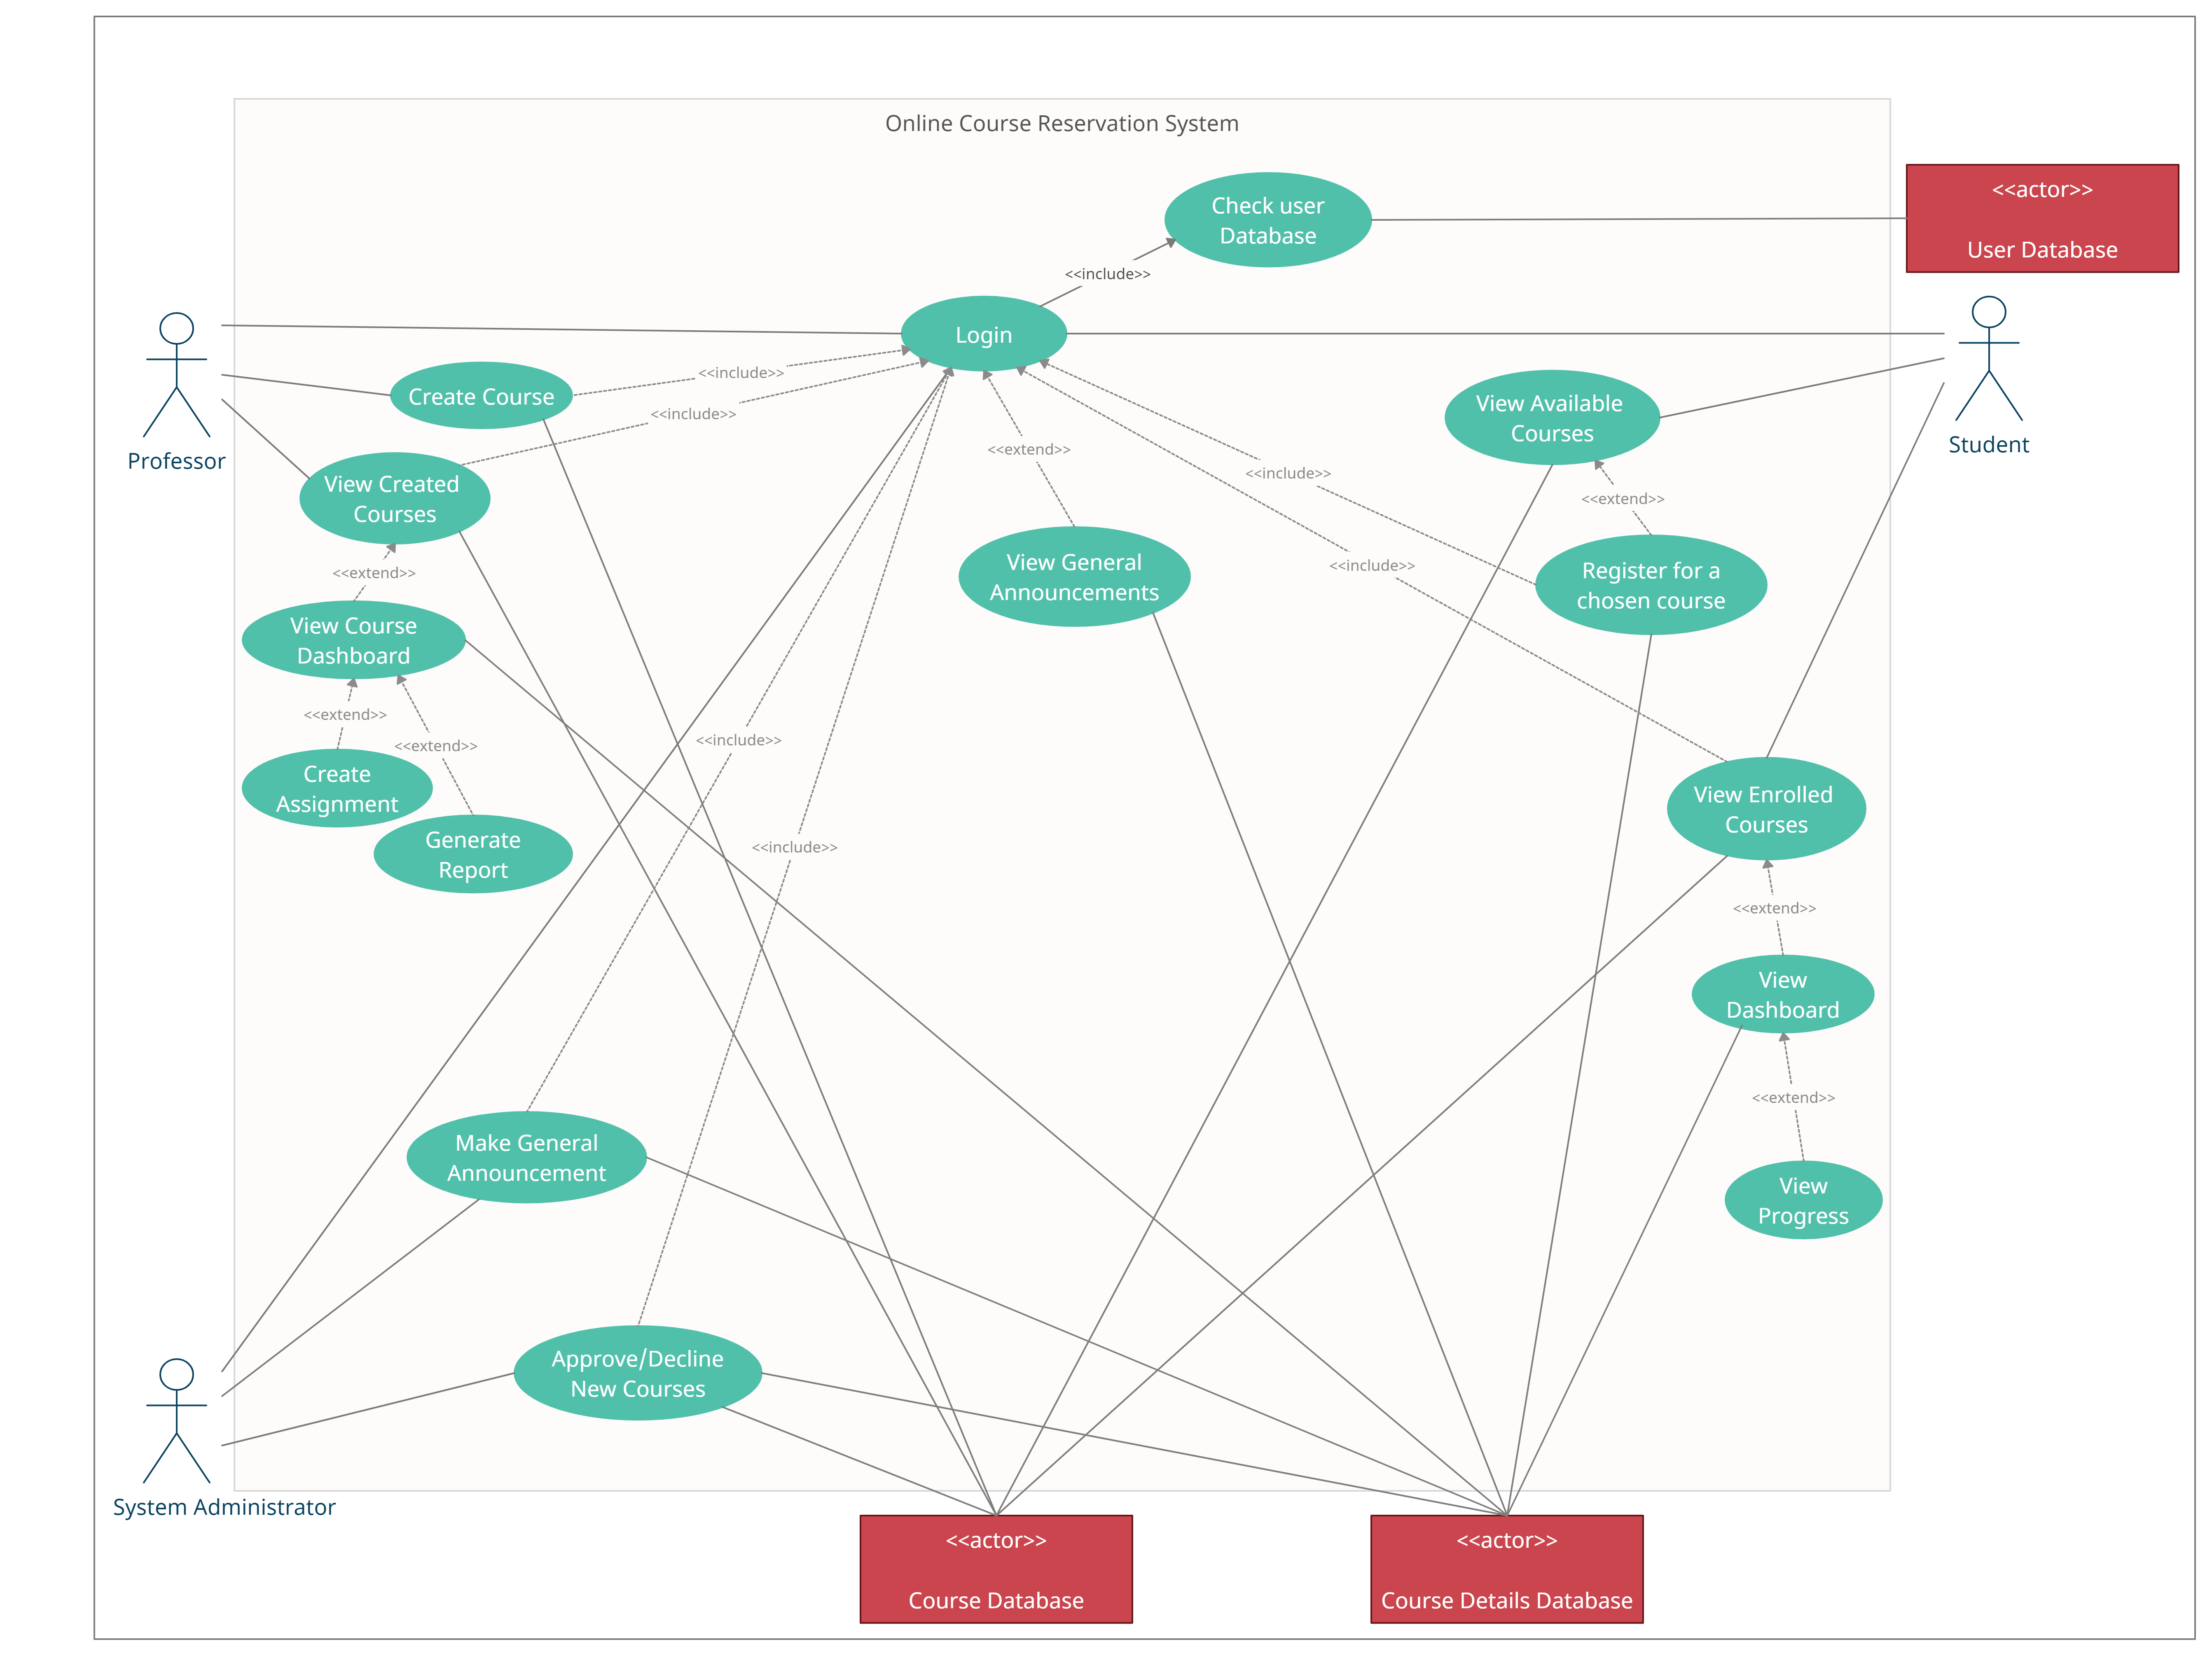
\includegraphics[width=\textwidth]{Use Case Diagram.png}
    \caption{Use Case Diagram for Online Course Reservation System}
\end{figure}

% --------------------------------------------------------------------------------------------------
% --------------------------------------------------------------------------------------------------

\newpage
\section{Use Case Descriptions}

% --------------------------------------------------------------------------------------------------

\subsection{Login}
\begin{itemize}
    \item \textbf{Overview}: This use case describes how a student, professor and system admin logs into the Course Reservation System.
    \item \textbf{Primary Actors}: Student, Professor and System Administrator
    \item \textbf{Secondary Actors}: User Database
    \item \textbf{Basic Flow}: This use case starts when an actor wishes to log into the Course Reservation System.
        \begin{enumerate}
            \item The system requests that the actor enter his/her name and password.
            \item The actor enters his/her name and password.
            \item The system validates the entered name and password and logs the actor into the system.
        \end{enumerate}
    \item \textbf{Alternative Flows}:
        \begin{enumerate}
            \item Invalid Name / Password \newline
            If in the Basic Flow the actor enters an invalid name and/or password, the system displays an error message. The actor can choose to either return to the beginning of the Basic Flow or cancel the login, at which point the use case ends.
        \end{enumerate}
    \item \textbf{Pre-Conditions}: None
    \item \textbf{Post-Conditions}: If the use case was successful, the actor is now logged into the system. If not the system state is unchanged.
    \item \textbf{Includes}: Check User Database
    \item \textbf{Extends}: View General announcements.
\end{itemize}

% --------------------------------------------------------------------------------------------------

\subsection{Check User Database}
\begin{itemize}
    \item \textbf{Overview}: Use case to Check User database.
    \item \textbf{Basic Flow}: This use case starts when an actor wishes to log into the Course Reservation System.
        \begin{enumerate}
            \item Give the User ID and Password
            \item Check if the user exists and the if password matches.
            \item Validate User entry
        \end{enumerate}
    \item \textbf{Alternative Flows}:
        \begin{enumerate}
            \item Invalid User ID: Produce Error: Invalid User ID Code
            \item Incorrect Password: Produce Error: Incorrect Password
        \end{enumerate}
    \item \textbf{Pre-Conditions}: None
    \item \textbf{Post-Conditions}: User is validated to login if success, not validated if any error is produced.
\end{itemize}

% --------------------------------------------------------------------------------------------------

\subsection{View General Announcements}
\begin{itemize}
    \item \textbf{Overview}: Use case to View General announcements made for the entire University.
    \item \textbf{Primary Actors}: Student, Professor and System Administrator
    \item \textbf{Secondary Actors}: Course Details Page
    \item \textbf{Basic Flow}: This use case starts upon request from any of the primary actors after they log into the system.
        \begin{enumerate}
            \item The system retrieves all general announcements from the Course Details Database and displays them.
        \end{enumerate}
    \item \textbf{Pre-Conditions}: The user must have logged into the system.
    \item \textbf{Post-Conditions}: None
    \item \textbf{Extends}: Login.
\end{itemize}

% --------------------------------------------------------------------------------------------------

\subsection{View Available Courses}
\begin{itemize}
    \item \textbf{Overview}: Use Case to view all available courses that the student can enroll for.
    \item \textbf{Primary Actor}: Student
    \item \textbf{Secondary Actor}: Course Database
    \item \textbf{Basic Flow}: This use case starts when an actor wishes to enroll in a new course.
        \begin{enumerate}
            \item The system retrieves all available courses from the Course Database
            \item The system displays them to the student allowing them to search and sort the list
        \end{enumerate}
    \item \textbf{Pre-Conditions}: None
    \item \textbf{Post-Conditions}: None
\end{itemize}
% --------------------------------------------------------------------------------------------------

\subsection{Register for a Course}
\begin{itemize}
    \item \textbf{Overview}: This use case describes how a student registers for a chosen course.
    \item \textbf{Primary Actor}: Student
    \item \textbf{Secondary Actors}: Course Details Database
    \item \textbf{Basic Flow}: This use case starts when an actor wishes to register for a course chosen from the available course list.
        \begin{enumerate}
            \item The user chooses the course they want to enroll in.
            \item The system retrieves the Course details and asks for confirmation.
            \item Login to the system if not already logged in.
            \item The Student confirms enrollment.
            \item The system updates the Course Details database with the new student.
        \end{enumerate}
    \item \textbf{Alternative Flows}:
        \begin{enumerate}
            \item The Student cancels enrollment.
            \item The System reverts back to displaying available courses.
        \end{enumerate}
    \item \textbf{Pre-Conditions}: Student must login to the system.
    \item \textbf{Post-Conditions}: If the use case was successful, the student is now enrolled in the system. If not the system state is unchanged.
    \item \textbf{Includes}: Login
    \item \textbf{Extends}: View Available Courses.
\end{itemize}

% --------------------------------------------------------------------------------------------------

\subsection{View Enrolled Courses}
\begin{itemize}
    \item \textbf{Overview}: Use Case to view all available courses that the student has already enrolled for.
    \item \textbf{Primary Actor}: Student
    \item \textbf{Secondary Actor}: Course Details Database
    \item \textbf{Basic Flow}: This use case starts when an actor wishes to view all their enrolled courses.
        \begin{enumerate}
            \item Login to the system if not already logged in.
            \item The system retrieves all courses that the student is enrolled in from the Course Details Database
            \item The system displays them to the student.
        \end{enumerate}
    \item \textbf{Pre-Conditions}: Student must login to the system.
    \item \textbf{Post-Conditions}: None
    \item \textbf{Includes}: Login.
\end{itemize}

% --------------------------------------------------------------------------------------------------

\subsection{View Course Dashboard (Student)}
\begin{itemize}
    \item \textbf{Overview}: Use Case to view the dashboard of a specific course the student has enrolled for.
    \item \textbf{Primary Actor}: Student
    \item \textbf{Secondary Actor}: Course Details Database
    \item \textbf{Basic Flow}: This use case starts when an actor wishes to go to the Dashboard of a course they have enrolled in.
        \begin{enumerate}
            \item The system retrieves information about the course and the student from the Course Details Database
            \item The system displays the information to the student.
        \end{enumerate}
    \item \textbf{Pre-Conditions}: Student must login to the system.
    \item \textbf{Post-Conditions}: None
    \item \textbf{Includes}: None
    \item \textbf{Extends}: View Enrolled Courses.
\end{itemize}

% --------------------------------------------------------------------------------------------------

\subsection{View Progress}
\begin{itemize}
    \item \textbf{Overview}: Use Case to view the progress of the student, i.e., marks, grades, attendance etc. in the chosen course.
    \item \textbf{Primary Actor}: Student
    \item \textbf{Secondary Actors}: Course Details Database
    \item \textbf{Basic Flow}: This use case starts when an actor wishes to view their progress in a chosen course.
        \begin{enumerate}
            \item The system retrieves information about the student's progress from the Course Details Database
            \item The system displays the information to the student.
        \end{enumerate}
    \item \textbf{Pre-Conditions}: Student must login to the system.
    \item \textbf{Post-Conditions}: None
    \item \textbf{Extends}: View Dashboard.
\end{itemize}

% --------------------------------------------------------------------------------------------------

% --------------------------------------------------------------------------------------------------

\subsection{Create Course}
\begin{itemize}
    \item \textbf{Overview}: This use case describes how a professor can create a course for the upcoming semester.
    \item \textbf{Primary Actor}: Professor
    \item \textbf{Basic Flow}: This use case starts when an actor wishes to create a new course for the upcoming semester.
        \begin{enumerate}
            \item The System requests the actor to enter the Name and syllabus of the new course.
            \item The System requests the actor to enter the intended semester when the students can take up the course
            \item The System creates a request to the system administrator to approve the course so that it can be added to the database
        \end{enumerate}
    \item \textbf{Pre-Conditions}: Professor must be logged into the system.
    \item \textbf{Post-Conditions}: A new course is sent for approval from the system administrator.
    \item \textbf{Includes}: Login
\end{itemize}

\subsection{View Created Courses}
\begin{itemize}
    \item \textbf{Overview}: Use case for a professor to view all courses they have created, to choose which one to manage.
    \item \textbf{Primary Actor}: Professor
    \item \textbf{Secondary Actor}: Course Database
    \item \textbf{Basic Flow}: This use case starts when an actor wishes to view all the courses they have created in order to manage any of them.
        \begin{enumerate}
            \item Gets \& Validates the Professor ID.
            \item Displays the catalog of all the courses and handled by the Professor.
        \end{enumerate}
    \item \textbf{Pre-Conditions}: Professor must login to the system.
    \item \textbf{Post-Conditions}: None
    \item \textbf{Includes}: Login.
\end{itemize}

\subsection{View Course Dashboard (Professor)}
\begin{itemize}
    \item \textbf{Overview}: Use Case to view the dashboard of a specific course the professor has created.
    \item \textbf{Primary Actor}: Professor
    \item \textbf{Secondary Actor}: Course Details Database
    \item \textbf{Basic Flow}: This use case starts when an actor wishes to go to the Dashboard of a course they have created.
        \begin{enumerate}
            \item The system retrieves information about the course from the Course Details Database
            \item The system displays the information to the professor.
        \end{enumerate}
    \item \textbf{Pre-Conditions}: Professor must login to the system.
    \item \textbf{Post-Conditions}: None
    \item \textbf{Includes}: None
    \item \textbf{Extends}: View Created Courses.
\end{itemize}

% --------------------------------------------------------------------------------------------------

\subsection{Create Assignment}
\begin{itemize}
    \item \textbf{Overview}: This use case describes how a professor can create an assignment for students taking up a specific course.
    \item \textbf{Primary Actor}: Professor
    \item \textbf{Secondary Actor}: Course Details Database
    \item \textbf{Basic Flow}: This use case starts when an actor wishes to create a new assignment for the students of the chosen course.
        \begin{enumerate}
            \item The System requests the actor to enter the Assignment Problem as a PDF.
            \item The System requests the actor to enter the deadline for the assignment.
            \item The System generates a post for the assignment given and posts it in the dashboard of the course
        \end{enumerate}
    \item \textbf{Pre-Conditions}: Professor must be logged into the system.
    \item \textbf{Post-Conditions}: A new assignment is issued and the details are posted in the dashboard of the course for all students to start working on it.
    \item \textbf{Includes}: Login
    \item \textbf{Extends}: View Course Dashboard (Professor).
\end{itemize}

% --------------------------------------------------------------------------------------------------

\subsection{Generate Report}
\begin{itemize}
    \item \textbf{Overview}: Use Case to view the report of a specific course the professor has created.
    \item \textbf{Primary Actor}: Professor
    \item \textbf{Secondary Actor}: Course Details Database
    \item \textbf{Basic Flow}: This use case starts when an actor wants to generate a report of all students that have taken the course.
        \begin{enumerate}
            \item The System retrieves all information about the course from the Course Details Database.
            \item The System calculates several statistical values for the marks and grades obtained by the students in the course such as mean, median etc.
            \item The System generates a report and displays it to the actor.
        \end{enumerate}
    \item \textbf{Pre-Conditions}: Professor must be logged into the system.
    \item \textbf{Post-Conditions}: A report is generated and displayed for the Professor
    \item \textbf{Includes}: Login
    \item \textbf{Extends}: View Course Dashboard (Professor).
\end{itemize}

% --------------------------------------------------------------------------------------------------

\subsection{Make a General Announcement}
\begin{itemize}
    \item \textbf{Overview}: This use case describes how the system administrator can make a general announcement for the entire system.
    \item \textbf{Primary Actor}: System Administrator
    \item \textbf{Secondary Actor}: Course Details Database
    \item \textbf{Basic Flow}: This use case starts when an actor wishes to make a new General Announcement.
        \begin{enumerate}
            \item The system administrator writes the General Announcement
            \item The System creates a post and displays the announcement in the General Announcements page (which is treated as a course with every student enrolled in it, and under every professor)
        \end{enumerate}
    \item \textbf{Pre-Conditions}: System Administrator must be logged into the system.
    \item \textbf{Post-Conditions}: A new general announcement is made.
    \item \textbf{Includes}: Login
\end{itemize}

% --------------------------------------------------------------------------------------------------

\subsection{Approve/Decline New Course}
\begin{itemize}
    \item \textbf{Overview}: This use case describes how the system administrator can either approve or decline a new course created by the professor.
    \item \textbf{Primary Actor}: System Administrator
    \item \textbf{Secondary Actor}: Courses Database and Course Details Database
    \item \textbf{Basic Flow}: This use case starts when an actor wishes to approve or decline a course pending approval in the system.
        \begin{enumerate}
            \item The System requests the system administrator to choose the pending course to take action for
            \item The System displays information of the course that the professor has entered.
            \item The System Administrator approves the course
            \item The System updates the Course Database and the Course Details Database with the new course.
        \end{enumerate}
    \item \textbf{Alternative Flows}:
        \begin{enumerate}
            \item The System Administrator declines the course
            \item The Professor is notified that the System Administrator has declined the course, the Databases remain unchanged
        \end{enumerate}
    \item \textbf{Pre-Conditions}: System Administrator must be logged into the system, and there must be pending courses to approve/decline.
    \item \textbf{Post-Conditions}: If the use case was successful, the course is now added to the system and the Course Database and the Course Details Database are updated. If not the system state is unchanged.
    \item \textbf{Includes}: Login
\end{itemize}

\end{document}